\documentclass[14pt]{mmcs_article}
\usepackage[russian]{babel}
\usepackage{amsmath, amsthm, amsfonts, amssymb}

%\graphicspath{{images/}}%путь к рисункам

\begin{document}

% Титульные листы
% раскомментировать требуемое
%%см. РЕКОМЕНДАЦИИ ПО ОФОРМЛЕНИЮ
%И ПРЕДСТАВЛЕНИЮ КУРСОВЫХ И ВЫПУСКНЫХ %КВАЛИФИКАЦИОННЫХ РАБОТ СТУДЕНТОВ ИНСТИТУТА %МАТЕМАТИКИ, МЕХАНИКИ И КОМПЬЮТЕРНЫХ НАУК


% ----------------------------------
% Внимание!
% Изменяйте только строки, перед которыми стоят знаки комментариев
% ----------------------------------

\thispagestyle{empty}
\begin{singlespacing}
\begin{center}

МИНОБРНАУКИ РОССИИ\\ [12pt]
Федеральное государственное автономное образовательное\\
учреждение высшего образования\\
<<Южный федеральный университет>>

\vspace{\baselineskip}
Институт математики, механики\\
и компьютерных наук им.~И.\,И.~Воровича

\vspace{\baselineskip}
% Название выпускающей кафедры
Кафедра алгебры и дискретной математики

\vfill
% Фамилия Имя Отчество студента
\textbf{Иванов Сергей Иванович}

\vspace{\baselineskip}
%%НАЗВАНИЕ РАБОТЫ должно полностью соответствовать распоряжению по Институту (для курсовых работ).
{\bf НАЗВАНИЕ РАБОТЫ, \\
РАЗБИТОЕ ПРИ НЕОБХОДИМОСТИ \\
НА НЕСКОЛЬКО СТРОК }

\vspace{15mm}
КУРСОВАЯ РАБОТА\\
по направлению подготовки\\
% указать направление обучения (раскомментируйте нужную строчку)
01.03.02~-- Прикладная математика и информатика
% 01.03.01~-- Математика
% 01.03.03~-- Механика и математическое моделирование 	
% 02.03.02~-- Фундаментальная информатика и информационные технологии


\vspace{10mm}
\textbf{Научный руководитель~--}\\
% указать данные о руководителе
% должность, степень, звание Фамилия Имя Отчество
проф., д.\,ф.-м.\,н. Сергеев Петр Сергеевич

\vspace{20mm}

\noindent
\begin{flushleft}
$\overline{\textrm{оценка (рейтинг)}}$\qquad	$\overline{\textrm{подпись руководителя\vphantom{й}}}$

\end{flushleft}


\vfill
% год!
Ростов-на-Дону -- 2020

\end{center}

\singlespacing
\end{singlespacing}  % для курсовой
%см. РЕКОМЕНДАЦИИ ПО ОФОРМЛЕНИЮ
%И ПРЕДСТАВЛЕНИЮ КУРСОВЫХ И ВЫПУСКНЫХ %КВАЛИФИКАЦИОННЫХ РАБОТ СТУДЕНТОВ ИНСТИТУТА %МАТЕМАТИКИ, МЕХАНИКИ И КОМПЬЮТЕРНЫХ НАУК


% ----------------------------------
% Внимание!
% Изменяйте только строки, перед которыми стоят знаки комментариев
% ----------------------------------

\thispagestyle{empty}
\begin{singlespacing}
\begin{center}

МИНОБРНАУКИ РОССИИ\\ [12pt]
Федеральное государственное автономное образовательное\\
учреждение высшего образования\\
<<Южный федеральный университет>>

\vspace{\baselineskip}
Институт математики, механики\\
и компьютерных наук им.~И.\,И.~Воровича

\vspace{\baselineskip}
% Название выпускающей кафедры
Кафедра информатики и вычислительного эксперимента

\vfill
% Фамилия Имя Отчество студента
\textbf{Волнобой Ирина Леонидовна}

\vspace{\baselineskip}
%НАЗВАНИЕ РАБОТЫ должно полностью соответствовать
% приказу по ЮФУ (для выпускных квалификационных работ)
{\bf РАЗРАБОТКА КОМПОНЕНТОВ ПРИЛОЖЕНИЯ \\
ДЛЯ АНАЛИЗА ОНЛАЙН-ПРОФИЛЯ \\
ЖИВОТНОГО ИЗ ПРИЮТА }


\vspace{15mm}
ВЫПУСКНАЯ КВАЛИФИКАЦИОННАЯ РАБОТА\\
по направлению подготовки\\
% Направление обучения
% раскомментируйте нужную строчку
02.03.02~-- Фундаментальная информатика и информационные технологии
% 01.03.01~-- Математика
% 01.03.02~-- Прикладная математика и информатика
% 01.03.03~-- Механика и математическое моделирование 	


\vspace{10mm}
\textbf{Научный руководитель~--}\\
% указать данные о руководителе
% должность, степень, звание Фамилия Имя Отчество 
доцент., к.\,ф.-м.\,н. Абрамян Анна Владимировна

\vspace{15mm}

\noindent
% указать Фамилию и инициалы 
% заведующего выпускающей кафедры
\begin{flushleft}
Допущено к защите:\\
заведующий кафедрой \underline{\hspace*{65mm}} Михалкович С.\,С.
\end{flushleft}




\vfill
% год!
Ростов-на-Дону -- 2021

\end{center}

\singlespacing
\end{singlespacing} % для работы бакалавра
%%см. РЕКОМЕНДАЦИИ ПО ОФОРМЛЕНИЮ
%И ПРЕДСТАВЛЕНИЮ КУРСОВЫХ И ВЫПУСКНЫХ %КВАЛИФИКАЦИОННЫХ РАБОТ СТУДЕНТОВ ИНСТИТУТА %МАТЕМАТИКИ, МЕХАНИКИ И КОМПЬЮТЕРНЫХ НАУК


% ----------------------------------
% Внимание!
% Изменяйте только строки, перед которыми стоят знаки комментариев
% ----------------------------------

\thispagestyle{empty}
\begin{singlespacing} 
\begin{center}

МИНОБРНАУКИ РОССИИ\\ [12pt]
Федеральное государственное автономное образовательное\\
учреждение высшего образования\\
<<Южный федеральный университет>>

\vspace{\baselineskip}
Институт математики, механики\\
и компьютерных наук им.~И.\,И.~Воровича


\vfill
% Фамилия Имя Отчество студента
\textbf{Иванов Сергей Иванович}

\vspace{15mm}
%НАЗВАНИЕ РАБОТЫ должно полностью соответствовать 
% приказу по ЮФУ (для выпускных квалификационных работ)
{\bf НАЗВАНИЕ РАБОТЫ, \\
РАЗБИТОЕ ПРИ НЕОБХОДИМОСТИ \\
НА НЕСКОЛЬКО СТРОК }

\vspace{15mm}
ВЫПУСКНАЯ КВАЛИФИКАЦИОННАЯ РАБОТА\\
по направлению подготовки\\
% Направление обучения 
01.04.02~-- Прикладная математика и информатика,\\
направленность программы\\
<<Математическое и программное обеспечение вычислительных машин>>

\vspace{10mm}
\textbf{Научный руководитель~--}\\
% указать данные о руководителе
% должность, степень, звание Фамилия Имя Отчество
проф., д.\,ф.-м.\,н. Сергеев Петр Сергеевич

\vspace{7mm}
\textbf{Рецензент~--}\\
% указать данные о рецензенте
% должность, степень, звание Фамилия Имя Отчество
доц., к.\,т.\,н. Петров Иван Петрович


\vspace{15mm}

\noindent
% указать Фамилию и инициалы руководителя
% образовательной программы
\begin{flushleft}
Допущено к защите:\\
руководитель \\
образовательной программы \underline{\hspace*{65mm}} Федоров Ф.\,Ф.
\end{flushleft}




\vfill
% год!
Ростов-на-Дону -- 2020

\end{center} 

\singlespacing
\end{singlespacing}% для работы магистра

\renewcommand{\contentsname}{Оглавление}

\tableofcontents

%=======================
\newpage
\addcontentsline{toc}{section}{Постановка задачи}

\section*{Постановка задачи}


В постановке задачи коротко (по пунктам) указывается, что необходимо сделать в рамках работы. Раздел <<Постановка задачи>> должен соответствовать заданию на курсовую или выпускную квалификационную работу, подписанному научным руководителем.


%=======================
\newpage
\addcontentsline{toc}{section}{Введение}
\section*{Введение}

Машинное обучение является одним из подразделов искусственного интеллекта. Оно нашло применение во многих сферах жизни: маркетинге, бизнесе, медицине, в банковской сфере, в различных научных исследованиях. Машинное обучение помогает в решении каких-либо вопросов, помогает принять решение, что нужно улучшить, чтобы увеличить или уменьшить какие-либо показатели и достигнуть цели. 

Например, в данной работе требуется на основе данных о питомцах предсказать, с какой скоростью животное будет принято в семью, а также какие признаки влияют на принятие решения в большей степени. Данная задача предложена к решению малайзийским сайтом petfinder.my. Сама задача, а также все необходимые данные представлены на ресурсе Kaggle [1]. Скорость в данной задаче является категориальной переменной, поэтому необходимо решить задачу классификации. Задача классификации является разновидностью задачи обучения с учителем и решается с помощью методов машинного обучения. 

Для решения данной задачи необходимо проанализировать исходные данные, выбрать наиболее подходящие для задачи методы обработки, применить различные алгоритмы машинного обучения, подобрать параметры, а также сравнить их качество и выбрать наиболее подходящий алгоритм, который показывает наилучшее качество на выбранной метрике.

В данной работе использовался язык программирования Python версии 3.8.2, библиотеки для визуализации matplotlib, seaborn, graphviz, библиотеки для обработки и анализа данных numpy и pandas, а также бибилотеки предоставляющие функционал для предварительной обработки данных и тренировки алгоритмов машинного обучения sklearn, XGBoost, LightGBM. В качестве инструмента для разработки использовался JupyterNotebook.

В качестве предварительной обработки данных использовались следующие методы: 
\begin{itemize}
	\item пропуски в данных заменены выборочным значением
	\item выбросы заменены выборочным значением или введена новая переменная, оценивающая исходную
	\item созданы новые признаки на основе имеющихся
	\item извлечены и обработаны признаки из данных, полученных от Google’s Natural Language API и от Google’s Vision API
	\item применены методы кодирования категориальных переменных: прямое кодирование, One Hot Encoding и Label Encoding
	\item данные приведены к одной шкале с использованием StandardScaler из sklearn
\end{itemize}

Создатели задачи рекомендуют к использованию метрику Quadratic Weighted Kappa, поэтому именно она используется для оценки качества моделей.

Для предсказания класса принятия на основе признаков были использованы алгоритмы логистической регрессии, дерева решений, случайного леса, а также три алгоритма градиентного бустинга из библиотек sklearn, XGBoost и LightGBM. Все модели и способы обработки были оценены и выбран наиболее оптимальный для данной задачи.

Также был использован алгоритм логистической регрессии с алгоритмом оптимизации стохастического градиентного спуска для предсказания целевой переменной на основе только текстовых признаков (описаний животных). Для этого описания животных были предварительно обработаны. Выполнена токенизация, нормализация, стемминг и лемматизация, векторизация методами Bags of Words и TF-IDF. Выполнен анализ эффективности модели на основе данных методов обработки текстов.

Настройка гиперпараметров моделей происходила по сетке с использованием GridSearchCV и RandomizedSearchCV из библиотеки sklearn.




%=======================
\newpage
\addcontentsline{toc}{section}{Обзор}
\section*{Обзор}

%=======================
\newpage
\section{Анализ исходных данных и их предварительная обработка}

\subsection{Описание поставленной задачи и исходных данных}

В данной работе использовались данные представленные на ресурсе Kaggle.  Это два основных датасета, представленных в формате csv:

\begin{itemize}
	\item train.csv --- содержит данные для тренировки модели размерностью 14993 записи на 25 столбцов.
	\item test.csv --- содержит данные для тестирования размерностью 3972 записи на 24 столбца. Данный датасет предназначен для тестирования модели на ресурсе Kaggle.
\end{itemize}

В train.csv на один столбец больше, чем в test.csv, так как тренировочный датасет содержит столбец AdoptionSpeed, который необходимо предсказать в тестовой выборке.

Так же имеется 3 csv файла, являющиеся словарями:

\begin{itemize}
	\item breed\_labels.csv --- словарь пород
	\item color\_labels.csv --- словарь окрасов шерсти
	\item state\_labels.csv --- словарь штатов
\end{itemize}

В словарях содержатся 2 колонки: id и расшифровка. Эти словари необходимы для лучшего понимания данных, так как в тренировочном и тестовом датасетах в колонках содержатся именно id пород, окрасов и штатов, а сами названия находятся в словарях.

Ещё имеются папка, содержащая метаданные, полученные с помощью Google’s Vision API с изображений, и папка, содержащая анализ тональности описаний, представленных в виде текста, который был получен с использованием Google’s Natural Language API. Эти данные представлены в формате PetID.json.

Вся информация, представленная в датасетах была взята создателями соревнования Kaggle с малайзийского сайта petfinder.my (рис. \ref{analyse:fig:1}). Это ресурс, главная задача которого состоит в том, чтоб найти новый дом животным. Анкеты животных на сайт выкладывают либо приюты, либо отдельные люди, которые нашли животное на улице. Несмотря на то, что на самом сайте представлены профили различных видов животных (попугаев, кошек, собак, хомячков, кроликов и так далее), в датасетах содержится информация только о профилях кошек и собак. На этом сайте люди имеют возможность отдать животное в хорошие руки бесплатно или же за определенную плату. Для этого создаётся профиль животного и добавляется туда информация о животном: фотография, кличка, возраст, пол, описание и другое.

\begin{figure}[H]
	\centering
	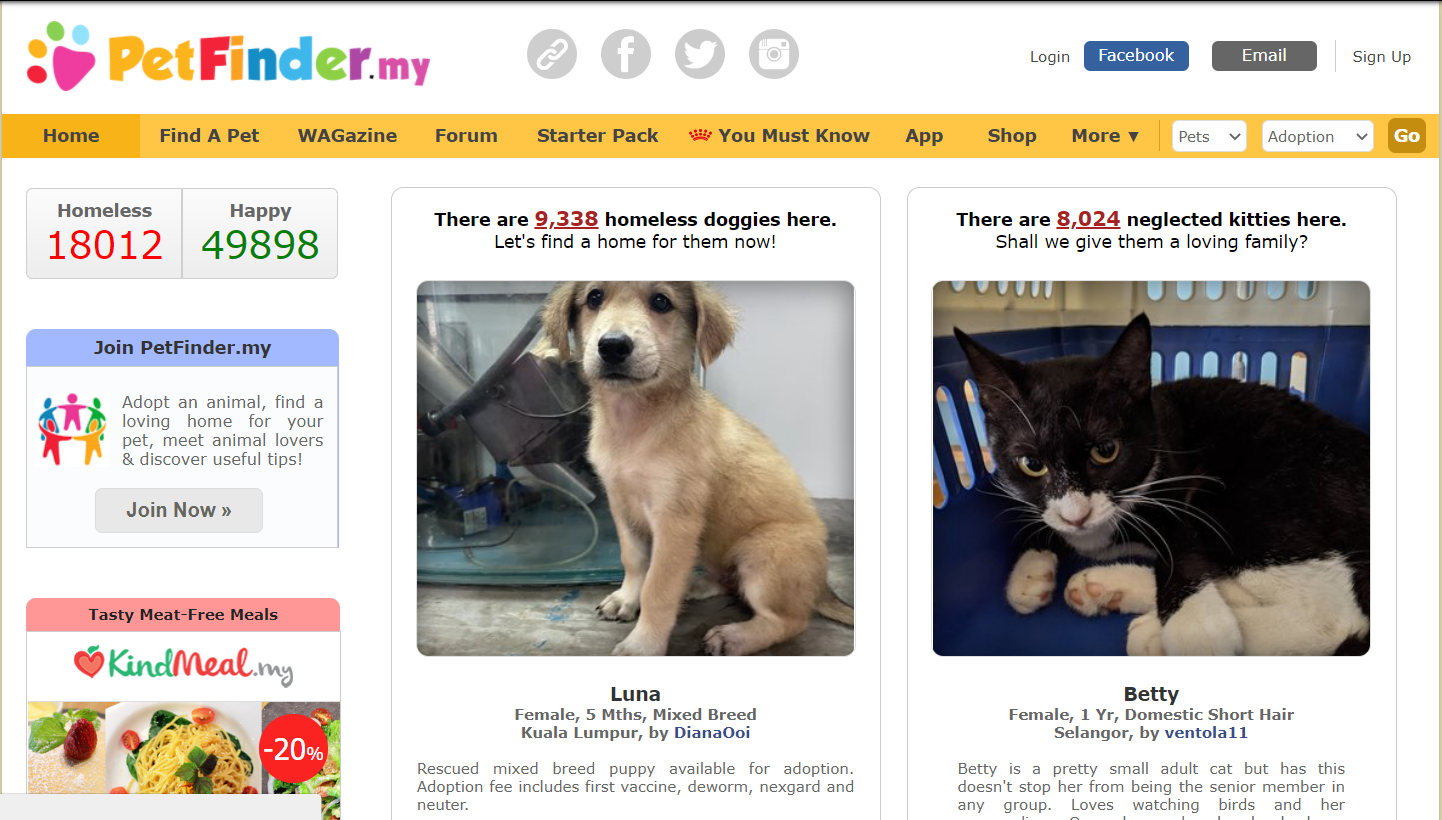
\includegraphics[scale=0.4]{petfinder}
	\caption{Скриншот сайта petfinder.my}\label{analyse:fig:1}
\end{figure}



\subsection{Описание признаков}

\subsection{Обработка пропущенных значений}

\subsection{Детекция и обработка выбросов}

\subsection{Создание новых признаков из имеющихся данных}

\subsection{Кодирование категориальных переменных}

\subsection{Шкалирование переменных}

%=======================
\newpage
\section{Используемая метрика}

%=======================
\newpage
\section{Использованные модели}

\subsection{Baseline}

\subsection{Дерево решений}

\subsection{Логистическая регрессия}

\subsection{Случайный лес}

\subsection{Градиентный бустинг}

%=======================
\newpage
\section{Классификация только с использованием текстовых признаков}

\subsection{Предобработка текстов и выделение признаков}

\subsection{Обучение модели}

\subsection{Полученные результаты}

%=======================
\newpage
\section{Выбор датасета, модели и тестирование на Kaggle}


%=======================
\newpage
\addcontentsline{toc}{section}{Заключение}
\section*{Заключение}

Заключение должно содержать информацию о проделанной работе и полученных результатах.

При написании текста работы следует иметь в виду, что её цель состоит в том, чтобы продемонстрировать квалификацию автора. Поэтому следует избегать общих и, тем более, тривиальных или нравоучительных высказываний. Мотивация выполняемой работы не должна носить слишком конкретный характер. Во время выступления на защите желательно избегать упоминаний об особенностях стандартных компонентов пользовательского интерфейса программ (<<нажимаем на правую кнопку>>, <<перетаскиваем фрагмент мышью>> и т.\,д.). Не следует комментировать задаваемые после защиты вопросы. Ответы на вопросы должны быть краткими.



%=======================
\newpage

\addcontentsline{toc}{section}{Литература}
\renewcommand{\refname}{\centering \textbf{Литература}}

\begin{thebibliography}{0}
\bibitem{stud:b0}
Рекомендации по оформлению
и представлению курсовых
и выпускных квалификационных работ
студентов института математики,
механики и компьютерных наук.~--
Ростов н/Д, 2020.

\bibitem{stud:b1}
Жуков М.\,Ю., Ширяева Е.\,В.
\LaTeXe: искусство набора и вёрстки текстов с~формулами.~-- Ростов н/Д : Изд-во ЮФУ, 2009.
\end{thebibliography}

%=======================
\newpage

\addcontentsline{toc}{section}{Приложение}
\section*{Приложение}



\end{document}
% ----------------------------------------------------------------


\lstset{ %
language=C++,                 % выбор языка для подсветки (здесь это С++)
basicstyle=\small\sffamily, % размер и начертание шрифта для подсветки кода
numbers=left,               % где поставить нумерацию строк (слева\справа)
numberstyle=\tiny,           % размер шрифта для номеров строк
stepnumber=1,                   % размер шага между двумя номерами строк
numbersep=5pt,                % как далеко отстоят номера строк от подсвечиваемого кода
backgroundcolor=\color{white}, % цвет фона подсветки - используем \usepackage{color}
showspaces=false,            % показывать или нет пробелы специальными отступами
showstringspaces=false,      % показывать или нет пробелы в строках
showtabs=false,             % показывать или нет табуляцию в строках
frame=single,              % рисовать рамку вокруг кода
tabsize=2,                 % размер табуляции по умолчанию равен 2 пробелам
captionpos=t,              % позиция заголовка вверху [t] или внизу [b]
breaklines=true,           % автоматически переносить строки (да\нет)
breakatwhitespace=false, % переносить строки только если есть пробел
escapeinside={\%*}{*)}   % если нужно добавить комментарии в коде
extendedchars=true,
commentstyle=\color{mygreen},    % comment style
stringstyle=\bf,
commentstyle=\ttfamily\itshape,
keepspaces=true % пробелы между русскими буквами
aboveskip=3mm,
belowskip=3mm

}


\renewcommand\NAT@bibsetnum[1]{\settowidth\labelwidth{\@biblabel{#1}}%
   \setlength{\leftmargin}{\bibindent}\addtolength{\leftmargin}{\dimexpr\labelwidth+\labelsep\relax}%
   \setlength{\itemindent}{-\bibindent+\fivecharsapprox}%
   \setlength{\listparindent}{\itemindent}
\setlength{\itemsep}{\bibsep}\setlength{\parsep}{\z@}%
   \ifNAT@openbib
     \addtolength{\leftmargin}{\bibindent}%
     \setlength{\itemindent}{-\bibindent}%
     \setlength{\listparindent}{\itemindent}%
     \setlength{\parsep}{0pt}%
   \fi
}
\renewcommand{\thesection}{\arabic{section}.}
\renewcommand{\thesubsection}{\arabic{section}.\arabic{subsection}.}
